\documentclass[a4paper,fleqn]{cas-dc}
\usepackage[numbers]{natbib}

\usepackage{mathtools}
\usepackage{booktabs}
\usepackage{flushend}
\usepackage{graphicx}
\usepackage{algorithm}
\usepackage{algorithmic}
\usepackage{amsmath}
\usepackage{amssymb}
\usepackage{tikz}
\usepackage{subcaption}

\numberwithin{equation}{section}

\begin{document}
\let\WriteBookmarks\relax
\def\floatpagepagefraction{1}
\def\textpagefraction{.001}

\shorttitle{Reliability Centric Network Design for Critical Wireless IoT Applications}
\shortauthors{Shettigar A. J. et al.}

\title[mode = title]{Reliability Centric Network Design for Critical Wireless IoT Applications}

\author[1]{Shettigar A.J.}[orcid=0009000942572756]
\cormark[1]
\ead{aditya.23mic7018@vitapstudent.ac.in}
\address[1]{School of Computer Science and Engineering, VIT AP University, Amaravati, Andhra Pradesh, India}

\cortext[cor1]{Corresponding author}

\begin{abstract}
With the emergence of wireless systems across many sectors of industry and other critical infrastructures, the issue of going beyond the simple connection to determinism and reliability became inevitable. The existing network topologies were designed for applications that would tolerate some packet losses and delays, which are totally unacceptable when dealing with power grid relays and robot arms on the assembly lines. This paper takes a cross-layer perspective on the analysis of factors influencing the success or otherwise of achieving reliability. The factors include node deployment, medium access control, physical layer propagation, and network architecture. The four areas of interest have had recent advancements in generative network-based topology optimization, grant-free coexistence of massive machine-type communications, propagation using intelligent surfaces, and distributed ledger robustness, respectively. In this paper, we develop a unified framework based on the aforementioned advancements. Through our simulation experiments carried out in Network Simulator Three, it is shown that the proposed framework results in high packet delivery rate and sub-millisecond delay under critical alarm burst conditions in dense mobile ad hoc networks of fifty nodes.
\end{abstract}

\begin{keywords}
Critical IoT \sep
Network Reliability \sep
Ad Hoc Networks \sep
Reactive Routing \sep
Deterministic Networking \sep
Self Healing Mesh \sep
Ultra Reliable Low Latency Communication \sep
Wireless Sensor Networks
\end{keywords}

\maketitle

\section{Introduction}

In contrast to simple consumers, such as smart home thermostat or wearable devices, nowadays wireless sensor technology is used in applications for which a delay or packet loss can be harmful – monetary or even human life. In fact, the operation of smart grids' substations, autonomous manufacturing lines, or remote surgical procedures requires a reliable delivery of information from sensors \cite{Chen_2021_Survey}. These kinds of applications are referred to collectively as Critical IoT, which is distinguished by the necessity of providing a deterministic communication path \cite{b7}.

Developing the system is rather challenging. The tough industrial conditions that characterize an environment, where the sensors work, entail a variety of channel impairments arising from the presence of multipath propagation through metal containers, wideband electrical noise produced by machines, as well as possible physical alterations that occur because of the factory layout modifications based on production-line requirements \cite{b1, Nawaz_2024_Backscatter}. Additionally, there is another problem associated with embedded hardware, namely its limited lifespan because of various vulnerabilities, among which are device aging, erroneous firmware, and overheating \cite{b6}. The standard parameters of performance evaluation, such as throughput and packet delivery ratio, are not designed to cope with stochastic breakdowns.

However, solving this issue would require an overhaul of the system design rather than improving the best effort technique currently in use. In this regard, this paper proposes an end-to-end cross-layer approach involving four distinct methods, which work together in solving this challenge. To begin with, the topology layer will utilize generative adversarial networks to ensure optimal positioning of sensor nodes, ensuring coverage and connectivity in spite of the malfunctioning of some sensors \cite{b2}. At the physical layer, reconfigurable intelligent surfaces will be used to manipulate the electromagnetic fields, overcoming the issue of signal blockages and fading caused by conventional antennas \cite{b4}.

Furthermore, at the MAC layer, grant-free contention schemes will be used together with reactive routing schemes like distance vector protocols to enable the co-existence of a massive number of mobile sensors along with critical low latency sensors \cite{b5}. Finally, at the architecture layer, a decentralized reliability protocol based on the distributed architecture will be employed to overcome the issue of centralization and mitigate the risk of a single point of failure in the gateway infrastructure \cite{b3}. This paper will be organized into six sections as follows. Section two will conduct a literature review and identify the research gap.

\subsection{Research Objectives}

Firstly, the first research goal is aimed at developing past static heuristic algorithms of sensor placement by applying generative modeling along with natural-inspired optimization algorithms to optimize the network topology in such a way that it provides maximal coverage and connectivity while being constrained in energy consumption by the battery power of wireless nodes \cite{b2, He_2025_GAN_Design}. The principle of operation of the proposed approach is in the ability of the generative network to model the statistics of the environment based on previous data and provide solutions to the optimization problem of network topology design which would not have been generated by conventional techniques such as particle swarm optimization or genetic algorithms.

Secondly, there is a necessity to develop access protocols and routing architectures for ensuring conflict-free access of machine-type communications of sensors and control traffic with sub-millisecond latency during alarm conditions \cite{b5, Ginige_2025_AdmissionControl, Popovski_2024_Slicing}. The application of grant-based access leads to latency during the handshake process. To solve this problem, the research will focus on the development of systems for grant-free access and routing which would provide a necessary delay guarantee when serving large amounts of devices in an environment consisting of fifty nodes.

The third aim is to integrate intelligent surfaces within the network structure so that the issue of signal blocking by the presence of many obstacles within the industrial environment gets sorted \cite{b4}. While active relay mechanisms require large amounts of energy consumption, intelligent surfaces or surface-based relaying techniques consume low energy and hence are cost-effective solutions in cases when incorporation of any new equipment would demand additional investment costs. This goal faces challenges pertaining to tuning of the phases of the relays in a way that ensures that the reflections occur in the same phase and thus form a line of sight connection between each other \cite{Wu_2024_RIS_Reliability, Chen_2024_RIS_Security}.

The fourth goal is to upgrade the vulnerable architecture that is used presently, namely, the one based on centralized gateway schemes, to a more secure one that relies on distributed ledgers for decentralized management and trust-building processes and that defines the concept of reliability in the terms of stochastic analysis so as to quantify the influence of node degradation and random errors \cite{b3, b6, Priyanka_2024_Synchronization}. This shift to distributed ledger-based mechanisms provides security guarantees because attacks against nodes do not affect the rest of the network while the shift away from probabilistic computations to stochastic analysis allows the framework to account for hardware deterioration and the geometry of failures on a mesh of nodes in space \cite{Shakhov_2024_LongWSN, Liu_2025_LinearWSN, Savadatti_2025_DLT_Survey, Shamir_2025_Blockchain_IoT}.

\section{Literature Survey}

In the last five years, many studies have been carried out in relation to wireless network reliability. Nevertheless, there is a lack of coherence in the field, as the optimization is generally carried out at one particular layer at a time, such as access control and physical propagation, without considering the interaction of other layers \cite{Chen_2021_Survey}. The fault tolerance experiments on industrial wireless sensor networks indicated that multipath routing and redundancy were useful in improving network reliability, although they were more reactive than preventive in their nature because they were done after detecting a network issue \cite{Ali_2021_Multipath}.

\subsection{Topology Optimisation and Physical Layer Hardening}

In looking at how the deployment of sensors developed through time, there is an obvious trend from deterministic approaches to much more dynamic, stochastic techniques that have become necessary due to the growing intricacy in industrial spaces. The early stages of IoT development focused on finding ways to implement geometric coverage using meta-heuristic techniques. Particle Swarm Optimization (PSO) and Genetic Algorithms (GAs) served as the preferred methods of optimization used for static deployments, where the optimization technique was employed within a predetermined environment with defined interference patterns, seeking out the "global optimum" between node density and signal power \cite{Moraes_2024_JointInterference, Nasir_2022_EnergyAware}.

Yet the contemporary industrial setting, which can be described as Industry 4.0 or 5.0, does not accommodate such approaches. Indeed, the factory floor of today is an arena of high-kinetic activity, where heavy equipment is modular and moved around frequently, Automated Guided Vehicles (AGVs) and mobile robotic arms navigate in irregular fashion, and structural divisions change depending on current needs. All of this leads to constantly changing Shadow Fading and Multipath Interference effects, which do not factor into a static PSO or GA approach.

In addition, with increasing node density towards the "Massive IoT" boundary condition, classical approaches for joint minimization of interference and power reach a point of the "computational wall," since the time necessary for computing all interference relations between nodes grows exponentially, resulting in unrealistic computation times and rendering such approaches useless in practice \cite{Moraes_2024_JointInterference}.

To tackle this issue related to the adaptability of classical approaches, a revolutionary concept has been put forward, the employment of the Generative Artificial Intelligence to model the domain of the problem. In other words, the task is not formulated as a mathematical task of solving an equation concerning nodes positioning, but rather is considered as a probability distribution of the functional layout. 

The recent advancements have proved that generative models such as Generative Adversarial Networks and Variational Autoencoders are capable of generating node topologies, which, interestingly enough, demonstrate intrinsic "fault tolerance." It means that the generated configuration would sustain functionality in case of multiple node failures or blocks, due to physical obstructions \cite{b2}.

Their usefulness has extended beyond the digital world of image generation. Recent advances show that GANs excel at creating intricate 3D layouts \cite{He_2025_GAN_Design}. Within industry, this implies planning the optimal location of nodes not only in two dimensions on a factory floor plan but also in three dimensions, considering multi-level assembly lines and overhead gantries. Three-dimensional awareness means the model can take advantage of vertical differences, meaning that while a ground-level connection may be obstructed by a passing forklift, an overhead relay node will continue transmitting the data flow.

The last step in the development of these designs is to integrate Adaptive Clustering into the process. Modern fault-tolerant architecture is dynamic, merging optimally placed physical layouts with logical clustering. In this case, each cluster is created with redundancy in mind, enabling it to "self-heal" in the event of malfunction or shielding of a node by a metallic object.

The lost capacity of any node is recovered through the ACapDS approach, which immediately takes up the traffic load of its neighboring nodes \cite{b7, Arapoglu_2024_ACapDS}. The combination of a physically generated structure and a logically evolving clustering layer guarantees the Massive IoT structure's resiliency, scalability, and capacity to support the sub-millisecond requirements of safety-critical cyber-physical systems.

There have been many advancements concerning intelligent surface technology in the critical environment at the physical layer. The general concept is that, given the use of meta-material components covering the surface, it is possible to generate reflections from any incoming signal, and then steer them to the targeted receiver even when direct line-of-sight connectivity is not available because of industrial equipment and steel structures \cite{b4}. The optimal design of the surface phase and transmit beamforming vectors will ensure substantial reduction in end-to-end latency and packet error rates that would satisfy safety-related applications \cite{Wu_2024_RIS_Reliability, Soleymani_2024_RIS_URLLC, Soleymani_2025_RSMA}.

Star reflective intelligent surfaces, which work for the devices on both sides of the panel, improve spectral efficiency for the cases where the panel must serve devices not visible at the same time \cite{Tahir_2024_STAR_RIS, Zhao_2024_DigitalTwin}. In particular, regarding the physical layer security, it could become an issue when a malfunctioning panel diverts sensitive information toward malicious eavesdropping nodes. This recent trend in the field has been looking at integrating the concept of physical layer security in the beamforming optimization problem \cite{Chen_2024_RIS_Security, Navarro_2024_StochasticBeamforming}. The combination of reflective surfaces and mobile edge computing with digital twins is beneficial for alleviating the computational complexity of real-time beamforming by offloading the task of beamforming computation from the resource-constrained nodes to the edge servers \cite{Antoniewicz_2024_Bandwidth, Mao_2024_Edge_Offloading}.

\subsection{Channel Coexistence and Network Architecture}

The channel coexistence issue can be classified into the allocation resource problem category. Machine-type communications deployments will be composed of thousands of sensors that periodically report their status updates, while few low-latency devices will require the channel to be available when they are ready to transmit their packets in critical situations such as industrial faults. Grant-based scheduling will be one solution, but its handshake process takes too long for low latency requirements. The admission control policies for next-generation networks and multi-access slicing for enhanced broadband with machine-type communications are two other notable examples of complexity \cite{Ginige_2025_AdmissionControl, Popovski_2024_Slicing}.

There are two possible alternatives for consideration, namely grant-free access and coded random access. In coded random access, the error correction coding approach is implemented at the access layer so that despite the presence of collisions, the receiver will be capable of decoding both packets via iterative decoding \cite{b5}. However, that is not sufficient, and if no reliable routing protocol exists, a broadcast storm will occur in just a few seconds for mobile nodes. The incorporation of reactive routing protocols would become the foundation of the solution \cite{Lin_2024_Reinforcement, Gholizadeh_2024_DRL_Reconfig}.

Architecture designs that utilize centralized architecture design, in which a sole gateway handles the entire network, have simple implementations; however, such a design presents significant risks to the security of the network since one hardware failure, software failure, or cyber attack can render the entire network useless. The solution lies in employing distributed reliability models, where the implementation of distributed computing design is incorporated in the design of the network management model, where all the nodes play an active role, and thus, no potential point of failure exists \cite{b3}. Self-healing algorithms based on deep reinforcement learning provide a complementary solution to the decentralized network architecture design, whereby the nodes dynamically find a path around network failures \cite{Wang_2025_DRL_SelfHealing}.

The use of distributed ledger technology (DLT) and blockchain architecture designs presents an extension of the concept of decentralization to include trust verification and auditing functionalities in the network. The traditional practice of undertaking such tasks within a central server is replaced by distributing such tasks among all nodes within a network and creating an immutable audit record using the shared ledger \cite{Savadatti_2025_DLT_Survey}. Such technology has been successfully applied in industrial networks to verify the integrity of sensor readings \cite{Rashid_2025_ZoneOfTrust}. Nonetheless, efficient implementation of the algorithm requires careful selection of a lightweight cryptographic scheme and consensus protocol with low computational overhead \cite{Wu_2025_LCAG, Hao_2024_DoubleBlockchain}.

\subsection{Reliability Metrics and Literature Summary}

Given the complexity of the problem space of Massive Internet of Things (MIoT) and mission-critical wireless sensor networks (WSN), an overall performance value in the form of average packet delivery ratio (PDR) in steady state cannot provide sufficient insight into the network's reliability. Though a network can have a PDR equal to ninety-nine percent in steady state, its hidden vulnerability could become apparent only under stress. The stress can occur when the system experiences a "dense burst," which is a synchronized stream of packets that emerge because of simultaneous activation of alarms or change to emergency state in the factory. Such events lead to an immediate buffer overflow and total channel contention, resulting in the network crash precisely during its peak efficiency period. Thus, analysis of such transient events is a necessary step for any infrastructure design \cite{b6}.

Reliability of the physical layer itself must be viewed from the perspective of dynamic reliability. Specifically, embedded system hardware and IoT device components are exposed to the risk of malfunction according to three major factors, which were identified within the reliability studies of IoT devices. The first factor is related to the presence of a bug in the node firmware, which could present the logical instability of the system, often leading to race conditions or memory leaks that trigger "silent" failures. Electrostatic discharge acts as an external shock, capable of permanently damaging delicate CMOS circuitry in industrial environments characterized by high electromagnetic noise. Finally, component aging—the gradual degradation of semiconductor materials and battery chemistry—ensures that the reliability of a node is a time-dependent function \cite{b1}.

In order to assess these risks, the analysis of reliability should extend from the “Average Case” to “Worst Case Execution” and “Survival Probabilities.” The MTTF of the components will be estimated by modeling the physical damage to the nodes through the Weibull distribution. At the same time, by carrying out the simulation of “catastrophic bursts” in the network routing layer, scientists can calculate the “saturation point,” at which the 99\% reliable network falls into near-availability. Such an approach provides for assessing reliability that takes into account not only random factors but also systematic impacts associated with large-scale application.

In Table \ref{tab:literature_summary}, a summary of the literature relevant to the proposed framework is provided. In this table, it is clear that there is always a trade off that is introduced with each layer contribution to the design. For instance, while the access layer reduces collisions, it also increases the transmission delay.

\begin{table*}[width=.9\textwidth,cols=5,pos=h]
\caption{Comparison of Reliability Centric Network Design Approaches}
\label{tab:literature_summary}
\begin{tabular*}{\textwidth}{@{\extracolsep{\fill}} p{0.15\textwidth} p{0.2\textwidth} p{0.2\textwidth} p{0.2\textwidth} p{0.2\textwidth}}
\toprule
\textbf{Ref.} & \textbf{Method Proposed} & \textbf{Techniques Used} & \textbf{Issues Resolved} & \textbf{Limitation} \\
\midrule

\cite{b2} &
Network Layout Optimisation &
Generative Adversarial Networks &
Poor sensor coverage and uneven energy usage &
Requires high computational power for generative training. \\
\addlinespace

\cite{b3} &
Distributed Reliable Architecture &
Distributed Computing &
Single point of failure in centralised controllers &
Complex data synchronisation across nodes. \\
\addlinespace

\cite{b4} &
Delay Minimisation via Surfaces &
Reconfigurable Intelligent Surfaces &
Signal blockage and high transmission latency &
High hardware cost for large scale surface deployment. \\
\addlinespace

\cite{b5} &
Coexistence Mechanisms &
Coded Random Access and Massive MIMO &
Data collisions between massive device populations &
Throughput degrades under extreme traffic loads. \\
\addlinespace

\cite{Wang_2025_DRL_SelfHealing} &
Self Healing Network Protocol &
Deep Reinforcement Learning &
Link failures caused by environmental changes &
Slow convergence in highly dynamic environments. \\
\addlinespace

\cite{b7} &
Fault Resilient Industrial Platform &
Redundant Node Deployment &
System downtime during hardware faults &
Increased deployment cost due to added hardware. \\

\bottomrule
\end{tabular*}
\end{table*}

\subsection{Research Gaps}

The analysis of the contemporary academic environment shows that there are still a number of unresolved problems within the framework of studies into MIoT and wireless networks in particular. Despite the emergence of innovative algorithms and approaches, the gap in the implementation of the solutions found appears to be rooted in a number of flaws in routing and medium access control optimization techniques, as well as the inefficiency of energy distribution within a system.

The main challenge associated with network optimization in \cite{b2} is the initial configuration of the network graph. In other words, although the algorithm in \cite{b2} demonstrates a substantial advancement in terms of the initial configuration of the spatial network structure, it does not address the fundamental problem of effective packet routing in an ever-changing topology. Namely, an industrial-scale network is constantly changing since nodes can easily malfunction, use up their energy resources, and even be relocated due to their attachment to the mobile robots. Under these circumstances, any initial configuration will inevitably become outdated due to the dynamic nature of the system. Therefore, the lack of integration between generative optimization algorithms and adaptive routing leads to the collapse of data transfer routes and loss of telemetry.

Similarly, things aren't looking any better on the MAC layer and routing layer. While the theoretical proof of coexistence without grants for machine type communication (MTC) and ultra-reliable low latency communication (URLLC) in the same radio channel, provided in \cite{b5}, can serve as a good starting point for efficient spectrum sharing, the ideal assumptions made in the proof cannot be realized in a multi-hop dense environment where broadcasting storms could easily cause the collapse of the system. Indeed, according to our simulation of fifty nodes deployed on a tight industrial floor, such a level of coexistence signaling may very well result in an exponentially increasing amount of broadcast traffic that will saturate the air and cause a great number of packet collisions, thus making all low-latency promises rendered meaningless. It is impossible for the coexistence protocol to function under the massive amount of broadcasting without a proper suppression mechanism.

Finally, the issue is equally severe in terms of security and energy consumption on the physical/architectural design layer. The design of \cite{b3} can be seen as a step in the right direction in acknowledging the extreme amount of energy waste associated with the consensus process in decentralized systems. Currently, there is no lightweight consensus approach that allows a resource-constrained node to validate a transaction or an identity within the ultra-tight time bounds required for real-time robotic actuation. The high computational jitter associated with decentralized trust means that we are often forced to choose between a secure but slow distributed system and a fast but vulnerable centralized one.

Lastly, the issue of the inability to conduct experiments using high-fidelity and realistic test environments is yet another important constraint. To validate the effectiveness of any newly proposed framework, one would need to conduct experiments on a simulated environment that mimics the "worst case" scenario of the industrial floor. However, as pointed out by \cite{b6}, such a model is extremely difficult to obtain due to the limitations that current simulations impose concerning alarm burst support. The problem here lies in the way in which most testing tools generate a traffic model that uses either Poisson distribution or a constant stream of alerts. In the real world, an emergency situation would generate an abrupt burst of several hundred alarms at once. This creates a nonlinear effect on the system that most tests conducted to date have failed to capture \cite{b6}. Unless a solution is found to incorporate such bursts into current tests, the "robustness" claims made by some authors are unrealistic in the context of the new infrastructure.

\subsection{Motivation}

The migration from consumer environments to critical environments is not a smooth progression but a paradigm shift regarding the consequences of errors. In a critical application using an autonomous assembly robot, a dropped packet could result in an injury in the workplace. Best-effort delivery schemes are ill-suited for such scenarios because of dynamic mobility, interference, and equipment degradation. Addressing this paradigm shift necessitates a radical departure from current wireless network topology, dynamic routing, and efficient handling of sudden bursts of critical alarms \cite{Chen_2021_Survey, b7}.

This problem was first motivated by the demand for five nines reliability and maximum delivery speed with sub-millisecond latency. All four objectives presented were motivated by gaps that can be addressed through the use of intelligent topology along with mesh routing to address mobility and error; access without grant to address latency; intelligent surfaces to deal with blockages; and ledger-based architecture to deal with the overhead required for security.

\subsection{Problem Statement}

The basic issue dealt with in this research is the lack of such an architecture of wireless sensor networks where all deterministic constraints can be satisfied simultaneously. The existing solution tries to optimize different criteria individually. The static scheme does not ensure self-correction of errors when faults happen and position changes take place \cite{b2}. For access layers, it is impossible to prevent collisions and packet loss if the number of nodes comes close to fifty, and frames with low latency cannot reach their deadlines within milliseconds \cite{b5}. The centralized control mechanism can be easily attacked and becomes a weak point in the whole production process \cite{b3}.

\section{Proposed Work}

This is implemented through a hierarchical stochastic cyber physical system, whose primary objective is to attain determinism in difficult industrial environments \cite{b7}. The network consists of various types of wireless nodes, ranging from massive machine-type nodes to ultra-reliable low-latency nodes. The framework is realized using four successive phases, which include topology synthesis, channel access control, post-quantum ledger consensus, and stochastic verification. The four phases rely on the result produced by their immediate predecessors, thus making them components of a single pipeline rather than independent modules.

\begin{figure*}[htbp]
\centering
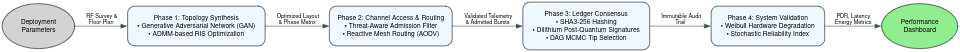
\includegraphics[width=\textwidth]{fig_overview_pipeline.png}
\caption{Four phase processing pipeline for critical environments.}
\label{fig:overview}
\end{figure*}

\subsection{Network Model}

All four phases utilize the network model to define the variables, channel models, nodes, and failure probabilities. By defining all of these at once, rather than throughout each phase subsection, it allows for mathematical dependence between the phases without repetition.

\subsubsection*{Network Topology and Node Types}

The area where deployment occurs is a crowded fifty-meter by fifty-meter floor of an industrial site. The sensor node transmits status information in the background while control nodes transport information having strict latency requirements of one millisecond at maximum. The routing layer ensures mesh connectivity through the use of reactive routing without causing any broadcast storms in case of changes in topology. A number of smart surface panels could be attached to columns in the building. All the elements’ shifts put together form the phase shift matrix:

\begin{equation}
\label{eq:ris_matrix}
\boldsymbol{\Phi} = \text{diag}\!\left(e^{j\theta_1},\, e^{j\theta_2},\, \dots,\, e^{j\theta_K}\right)
\end{equation}

\subsubsection*{Channel Model}

The signal received at the distributed edge receiver from a node combines the direct propagation path, the reflected path, inter node interference, and thermal noise \cite{b4}:
\begin{equation}
\label{eq:received_signal}
y_i(t) = \Bigl(\boldsymbol{h}_{d,i} + \boldsymbol{h}_{r,i}^{T}\boldsymbol{\Phi}\,\boldsymbol{g}\Bigr)\,x_i(t) + \sum_{j \neq i} I_j(t) + n_0(t)
\end{equation}
The signal to interference plus noise ratio at the receiver for the node follows directly from the signal equation:
\begin{equation}
\label{eq:sinr}
\text{SINR}_i = \frac{\bigl|\boldsymbol{h}_{d,i} + \boldsymbol{h}_{r,i}^{T}\boldsymbol{\Phi}\,\boldsymbol{g}\bigr|^2 P_i}{\displaystyle\sum_{j \neq i}\left|h_j\right|^2 P_j + \sigma^2}
\end{equation}
End to end packet delay for an admitted critical burst must reliably satisfy the maximum limit:
\begin{equation}
\label{eq:latency}
D_{e2e} = D_{prop} + D_{proc} + D_{queue} \leq L_{max}
\end{equation}

\subsubsection*{Threat Model}

Every incoming packet burst passes through an intrusion detection function before processing begins. The admission decision checks the threat threshold:
\begin{equation}
\label{eq:watchdog}
\mathcal{W}\!\left(B(t)\right) =
\begin{cases}
1, & \mathbb{P}\!\left(\text{Malicious}\mid\text{Features}\right) < \tau_{th} \\
0, & \text{otherwise}
\end{cases}
\end{equation}
When the burst is quarantined, data integrity is anchored in a directed acyclic graph distributed ledger \cite{b3}. Each transaction is signed with a lattice based post quantum signature. The probability that an adversary with a quantum computer forges a valid signature is bounded by:
\begin{equation}
\label{eq:forge_prob}
\mathbb{P}_{\text{forge}}\!\left(\mathcal{A}_{PQ}\right) \leq \epsilon_{PQ}
\end{equation}

\subsubsection*{Reliability Model}

Node survival is modelled with a Weibull distribution to capture how hardware degradation accelerates over operating time \cite{b6, b1}:
\begin{equation}
\label{eq:weibull}
R_i(t) = \exp\!\left(-\!\left(\frac{t}{\eta_i}\right)^{\!\beta_i}\right)
\end{equation}
Assuming statistically independent node failures, the system level reliability is computed as the product of all nodes:
\begin{equation}
\label{eq:system_reliability}
R_{sys}(t) = \prod_{i=1}^{|\mathcal{N}|} \exp\!\left(-\!\left(\frac{t}{\eta_i}\right)^{\!\beta_i}\right)
\end{equation}

\subsection{Phase 1 Topology Synthesis}

The spatial dynamics of modern industrial factories' floor layouts consist of a chaotic coordination between massive machines, mobile robotic units, and dense metallic structures, creating an RF environment characterized by non-stationarity and extremely difficult conditions for IoT sensor networks deployment. The positioning of such networks in a chaotic RF environment implies not only logistical challenges but rather an engineering limitation that directly impacts the operational lifetime of each individual IoT node and its ability to remain reliable in operation. A wrongly positioned node will face difficulties caused by multipath fading and dynamic obstructions, compelling it to boost the output power to compensate for the losses during excessive multi-hop transmissions. Thus, "power creep" will quickly drain the limited energy resources of a node, reducing its operational lifetime from several years to just a few months. As a consequence, a "domino effect" of coverage holes appears, generating "dark zones" within the overall area covered by the IoT node network on the factory floor.

To overcome these challenges, the first phase of the proposed architecture incorporates a robust Generative Adversarial Network (GAN) model, transcending the limits of heuristic methods of deploying IoT networks in a dynamic environment. In general, the traditional approach often rely on a "best-guess" approach or simple Voronoi tessellation, which fail to capture the stochastic nature of an industrial floor where a 10-ton overhead crane or a new assembly line partition can instantly sever a communication link. 

The Generative Model in this architecture serves as an artificial architect. The model consumes huge amounts of data in the form of Signal-to-Noise Ratio (SNR) heat maps, Packet Delivery Ratio (PDR) logs, and physical coordinates. Through its analysis, it recognizes the latent "statistics" of the particular deployment environment in terms of blockages. It detects the correlation between operating hours of certain machines and RF attenuation in the network. For example, the model may recognize that once a particular hydraulic press begins operation, the resulting EMI makes communication impossible through low-power Zigbee or 6LoWPAN in certain coordinate ranges.

The Discriminative Model acts as a tough "adversary" or critic in this case. Its purpose is simple - determine whether the proposed node deployment scenario is "viable" or not from the perspective of reliability (in other words, if the required 99.999\% reliability is provided). Therefore, the competition pushes the generative model to come up with more complex topologies that ensure high reliability even when all possible worst-case scenarios occur, such as failure of both a gateway and primary relay node.

Moreover, a generative model enables us to create simulations of "What-If" scenarios. Without any physical installation of the nodes, the GAN will already be able to come up with thousands of coordinate combinations and test them for potential errors. This way we get a "Probability of Connectivity" graph that will direct us in terms of which location of the nodes will make the network the most resilient. Optimization of the physical layer installation using such a machine learning approach results in an inherent increase in the energy efficiency of the network. As each individual node in our network operates at the optimal, minimal transmit power level, the life expectancy of all nodes in our MIoT network is maximized while there will not be any coverage holes in the industrial cycle \cite{b2}.

The resulting network layout is an instance of proactive networking. Unlike "best-effort" connectivity, in which we respond to the signal loss by increasing power and wasting more resources (in both the short and long term), a solution with GAN-generated coordinates provides us with a "physical skeleton" of the network built on the grounds of its electromagnetic geography. Thus, we are making the crucial leap from best-effort wireless connectivity towards deterministic wireless engineering, providing the stable foundation necessary for Stage 2’s higher-level security and anomaly detection protocols. The training objective balances coverage against energy. The generator loss and discriminator loss follow the standard minimax formulation:
\begin{equation}
\label{eq:gan_loss}
\min_{G}\max_{D}\; \mathbb{E}_{\mathcal{X}\sim p_{data}}\!\left[\log D(\mathcal{X})\right] + \mathbb{E}_{z\sim p_z}\!\left[\log\!\left(1 - D(G(z))\right)\right]
\end{equation}
The fraction of grid points that satisfy the minimum requirement defines the coverage metric:
\begin{equation}
\label{eq:coverage}
C(\mathcal{X}_{cand}) = \frac{1}{N_g} \sum_{k=1}^{N_g} \mathbf{1}\!\left[\text{SINR}_k\!\left(\mathcal{X}_{cand}\right) \geq \gamma_{\min}\right]
\end{equation}

Algorithm one details the generative layout procedure. Once the model converges on an optimal layout, an alternating direction method of multipliers solver tackles the quadratically constrained quadratic program to find the phase configuration that maximises the effective reflected channel gain \cite{b4}:
\begin{equation}
\label{eq:qcqp}
\max_{\boldsymbol{\Phi}}\;\left|\boldsymbol{h}_{r,u}^{T}\boldsymbol{\Phi}\,\boldsymbol{g}\right|^2 \quad \text{subject to}\quad |\theta_k| = 1
\end{equation}
The total energy expended across the deployment is minimised by favouring compact topologies, directly extending the useful life of every battery powered node:
\begin{equation}
\label{eq:energy}
E_{total} = \sum_{i \in \mathcal{N}} P_i \cdot T_{active,i}
\end{equation}

\begin{algorithm}[!ht]
\caption{Generative Network and Intelligent Surface Optimization}
\label{alg:topology}
\begin{algorithmic}[1]
\renewcommand{\algorithmicrequire}{\textbf{Input:}}
\renewcommand{\algorithmicensure}{\textbf{Output:}}
\REQUIRE Floor plan, survey data, coverage target, signal threshold, maximum epochs, minimum tolerance
\ENSURE Optimal node layout, surface phase matrix
\STATE Initialise Generator network parameters
\STATE Initialise Discriminator network parameters
\STATE Pre process survey data into volumetric occupancy grid
\STATE Set epoch counter to zero
\WHILE{epoch less than maximum epochs and loss has not converged}
\STATE Sample noise vector conditioned on floor plan
\STATE Generate candidate layout from noise vector
\STATE Compute interference map over observation grid
\STATE Compute coverage score across all observation points
\IF{coverage score less than target}
\STATE Assign negative training label to candidate layout
\ELSE
\STATE Assign positive training label to candidate layout
\ENDIF
\STATE Update Discriminator by minimising standard loss
\STATE Update Generator by maximising discriminator score
\STATE Increment epoch counter
\ENDWHILE
\STATE Extract optimal layout from converged model
\STATE Initialise surface phase shifts to identity configuration
\STATE Set iteration counter to zero
\WHILE{primal residual greater than minimum tolerance}
\STATE Apply semi definite relaxation to modulus constraints
\STATE Solve relaxed quadratic program for phase matrix
\STATE Project resulting matrix onto feasible modulus set
\STATE Update dual variables for coupling constraints
\STATE Increment iteration counter
\ENDWHILE
\RETURN Optimal node layout, converged phase matrix
\end{algorithmic}
\end{algorithm}

\subsection{Phase 2 Channel Access and Routing}

Once the topology is physically configured and the geographical coordinates established during the generation phase, attention turns to the live operation stage where the access and routing layers will be handling highly mobile and fast-moving traffic. In phase two, a unique MANET design customized for Massive IoT is introduced. The main issue in wireless sensor networks with high node density is the broadcast storm, whereby repeated transmissions of route request (RREQ) packets exhaust the channel’s capacity leading to numerous packet collisions, thus paralyzing the entire network. To avoid this scenario, the suggested system adopts a MANET network architecture in combination with a highly effective reactive routing algorithm, more precisely the adapted Ad hoc On-demand Distance Vector (AODV) routing protocol, which differentiates between normal and emergency data.

The design is such that there is no need to have a globally static routing table due to the computational complexity involved, which quickly becomes obsolete in the case of mobile communication. The reactive approach, in this case, ensures that route discovery occurs when there is an actual need to send packets by individual nodes. The process thus reduces the cost involved in route exploration. To minimize broadcast storms, the approach involves a probabilistic broadcasting approach, and at the same time takes into account the information regarding neighborhood traffic load. In this case, nodes first check the traffic load and their current battery life. If a node is either congested or lacks energy, the process of broadcasting is prevented.

Simulation setting puts an extremely stressful load on the logic proposed, as in a grid with the size of 2,500 square meters (that equals to fifty meters by fifty meters). In such an area, mobility of the nodes will be based on the Random Waypoint (RWP) Mobility Model. This implies that nodes select a random destination point and proceed to it using pre-defined velocity, followed by a "think time," during which a new destination is chosen. Such a pattern of movement mimics behavior of automated guided vehicles (AGVs) and mobile robots that operate around static assembly lines. During the course of such dynamic events, constant reconfiguration of links and routes, referred to as "link repair" and "route maintenance," becomes necessary.

In the middle of this grid, exactly at coordinate (25, 25), is located the only edge gateway, which serves as a fixed sink of the sensor data and a connection point to cloud controller. It is done mathematically correct, since placing the edge gateway closer to the corners would increase the maximum hop count and result in larger overall latency and increased probability of packets being lost during the transmission due to high hop count. At the same time, keeping the gateway fixed while the surrounding nodes remain highly mobile, the simulation forces the routing layer to continuously adapt to changing "next-hop" candidates.

Such an adaptive mechanism helps create a self-organized fabric for the network. This enables large-scale sensors that could be sending packets every few minutes about their readings to exist harmoniously with actuators that need millisecond reaction times. Prioritization of critical packets is achieved by using the Multi-Level Priority Queue (MLPQ) mechanism within the MAC layer; critical information is sent before telemetry. As a result, despite being in a highly mobile and interference-prone environment, the backbone communication system remains resilient, flexible, and immune to catastrophic traffic jams that are associated with generic IoT networks.

\begin{figure}
\centering
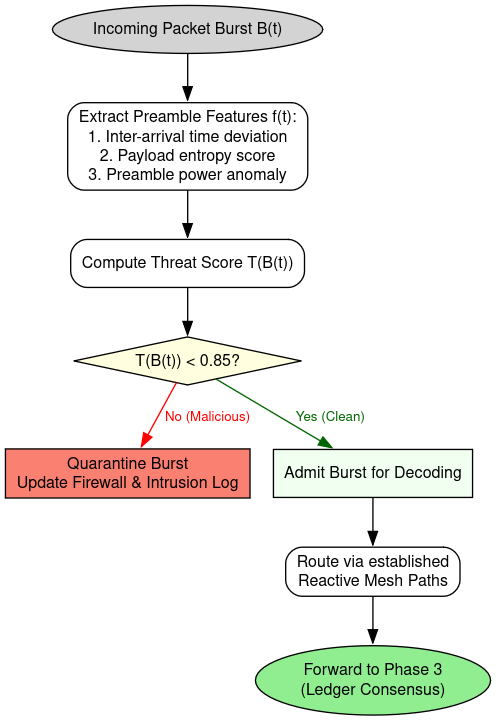
\includegraphics[width=\linewidth]{fig_phase2_mac.png}
\caption{Access layer operation showing grant free coexistence.}
\label{fig:mac_layer}
\end{figure}

The received composite signal at the base station is the superposition of all active node transmissions:
\begin{equation}
\label{eq:composite}
y(t) = \sum_{i \in \mathcal{N}_U} y_i(t) + \sum_{m \in \mathcal{N}_M} y_m(t) + n_0(t)
\end{equation}

Algorithm two outlines the access control logic. To secure the flow, before any decoding happens, the intrusion detection function scores the incoming burst. The threat score uses a three feature vector extracted from the packet preamble:
\begin{equation}
\label{eq:threat}
\mathcal{T}(B(t)) = \mathbb{P}\!\left(\text{Malicious}\mid f_1(t),\, f_2(t),\, f_3(t)\right)
\end{equation}
The false positive rate of this classifier is bounded to protect throughput:
\begin{equation}
\label{eq:fpr}
\text{FPR} = \frac{FP}{FP + TN} \leq \delta_{FP}
\end{equation}
Once validated, packets are dynamically routed to the edge gateway via the established mesh paths. This reactive approach ensures that as mobile nodes traverse the grid, the routing table updates gracefully without saturating the channel bandwidth.

\begin{algorithm}[!ht]
\caption{Threat Aware Admission and Routing Validation}
\label{alg:mac}
\begin{algorithmic}[1]
\renewcommand{\algorithmicrequire}{\textbf{Input:}}
\renewcommand{\algorithmicensure}{\textbf{Output:}}
\REQUIRE Incoming packet burst, security threshold, error bound
\ENSURE Validated symbols, updated routing paths
\STATE Extract preamble timing vectors from incoming burst
\STATE Extract payload entropy vectors from incoming burst
\STATE Extract power anomaly vectors from incoming burst
\STATE Aggregate vectors into comprehensive feature matrix
\STATE Compute probabilistic threat score using feature matrix
\IF{threat score greater than or equal to security threshold}
\STATE Flag incoming burst as highly malicious
\STATE Record anomaly event in local security memory
\STATE Isolate transmitting source node from network
\STATE Update dynamic firewall ruleset configuration
\STATE Increment intrusion detection logging counters
\RETURN Null set
\ENDIF
\STATE Flag incoming burst as safe for processing
\STATE Validate operational error rate against error bound
\IF{operational error rate exceeds error bound}
\STATE Trigger system calibration warning flag
\ENDIF
\STATE Accept packet burst into baseband decoding module
\STATE Extract intended destination address from headers
\STATE Lookup reactive mesh routing paths locally
\IF{valid routing path is not currently found}
\STATE Initiate reactive route discovery sequence globally
\ENDIF
\STATE Forward packet payload to designated next hop
\STATE Record latency metrics for performance logging
\STATE Verify strict delivery deadline constraints
\RETURN Decoded symbols
\end{algorithmic}
\end{algorithm}


\subsection{Phase 3 Ledger Consensus}

The final and the most crucial stage of the security pipeline consists of the shift from active routing to persistence layer. Indeed, all telemetry records, whether they represent regular readings or mission-critical actuator commands, which have managed to successfully reach Phase Two, automatically enter Phase Three and get permanently and cryptographically immortalized through the process of persistent storage in a DAG ledger. These records are no longer simply stored in a typical and easily hackable SQL database. On the contrary, they get permanently recorded in a ledger designed on the basis of the Distributed Acyclic Graph model. In contrast to conventional blockchain ledgers, DAG-based ledger does not require any synchronous validations, which results in a high level of latency. The latter, in its turn, makes DAG-based ledger architecture particularly suitable for use with the Massive IoT paradigm.

There are two core reasons for using a DAG blockchain ledger. First, it allows for generating a mathematically immutable audit trail which can be used both by the regulators and independent industry auditors. For example, in the case of smart healthcare and other industries, it is vital to prove that a certain order was given from a certain authorized node with mathematical certainty in case of an incident. The second reason why we use DAG is that the decentralized approach allows us to avoid a single point of trust (SPOF). In classical centralized solutions, the corruption of the central database server means that the integrity of all records from its history is compromised in case of DDoS attacks. However, in a decentralized environment, the truth about sensor records is split between several edge nodes and clouds.

Yet, the critical breakthrough in Phase Three comes from the use of a new cryptographic foundation. Traditional distributed ledgers employ Elliptic Curve Cryptography (ECC) to ensure that the transactions on their networks are protected via encryption algorithms such as ECDSA. The security of ECC is based on the mathematical complexity of the Discrete Logarithm Problem (DLP). ECC is resilient to the classical supercomputer but can easily be broken by Shor’s algorithm on a quantum machine. Hence, depending on ECC for the long-term sustainability of a network is like "putting yourself on the ticking time bomb" in terms of cryptography.

Phase Three resolves this problem by switching to a novel Lattice-Based Signature Scheme that uses a different cryptographic framework. The signature scheme employed in Phase Three does not depend on DLP but rather relies on the Learning With Errors (LWE) problem—one of the fundamental problems of post-quantum cryptography. The lattice problem is believed to be computationally hard even when run on a classical or quantum machine since it involves computing the shortest vector in a large point set. Hence, by adopting the lattice-based cryptographic framework, Phase Three provides long-term security to the MIoT ecosystem in the Post-Quantum era and protects it. By utilizing this lattice-based approach, the architecture ensures that the MIoT ecosystem remains secure in the "Post-Quantum" era, neutralizing the threat of "harvest now, decrypt later" attacks by nation-state actors.

Also, the design of this signing process is carefully fine-tuned to guarantee the desired level of forge-proofing in order to protect from attackers during the execution of industrial-scale processes. Given the size of the network, the possibility of forging the signature of an object through the brute force or mathematical attacks should be minimal ($2^{-128}$ or smaller). However, the size of the cryptographic signature has to correspond to its level of resistance, which is guaranteed by the selection of parameters of the lattices used in this framework (i.e., the dimension and noise in the sample of the LWE problem). As opposed to ECC signatures, lattice-based ones tend to be bigger in size; yet, Gaussian sampling and Rejection Sampling are applied to make them small enough to fit in the limited MTU of the IoT packets.

Thus, this phase turns unfiltered telemetry into meaningful and secured information. At the end of this pipeline, the packet will have gone through physical optimization of placement (Phase One), self-organization-based routing (Phase Two), and cryptographic anchoring to an immutable, post-quantum ledger (Phase Three). This way, this technology ensures the full potential of a Zero-Trust Wireless Architecture.

\begin{figure}
\centering
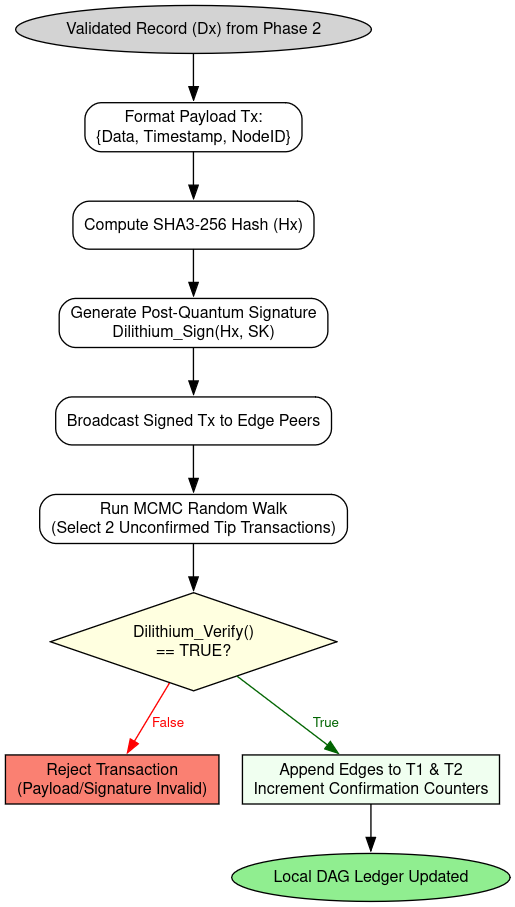
\includegraphics[width=\linewidth]{fig_phase3.png}
\caption{Post Quantum Ledger Consensus Integration.}
\label{fig:fsm}
\end{figure}

The ledger is a graph where each vertex holds one signed transaction record. Algorithm three details the attachment sequence. A new transaction is attached by referencing two existing unconfirmed tip transactions from the frontier. Tip selection follows a random walk weighted by cumulative vertex confirmation counts:
\begin{equation}
\label{eq:dag_weight}
W(v) = \sum_{w:\, v \rightarrow w} c(v,\, w)
\end{equation}
The cryptographic hash of each transaction payload is computed and the complete signed transaction object is structured to ensure post quantum verification returns true before acceptance:
\begin{equation}
\label{eq:verify}
\text{Dilithium\_Verify}\!\left(H_x,\, \Sigma_x,\, PK_{PQ}\right) = \text{TRUE}
\end{equation}

\begin{algorithm}[!ht]
\caption{Post Quantum Ledger Consensus Integration}
\label{alg:ledger}
\begin{algorithmic}[1]
\renewcommand{\algorithmicrequire}{\textbf{Input:}}
\renewcommand{\algorithmicensure}{\textbf{Output:}}
\REQUIRE Validated record, private key, distributed graph ledger
\ENSURE Updated global ledger state
\STATE Format transaction payload including data contents
\STATE Append creation timestamp to transaction payload
\STATE Append node identifier to transaction payload
\STATE Compute secure cryptographic hash of entire payload
\STATE Generate post quantum digital signature using hash
\STATE Construct complete signed transaction object array
\STATE Broadcast transaction array to neighbouring edge peers
\STATE Initialize cumulative weights for all active vertices
\STATE Compute connection weights based on historical paths
\STATE Execute first random walk originating from genesis block
\STATE Set first reference tip transaction node
\STATE Execute second random walk originating from genesis block
\STATE Set second reference tip transaction node
\STATE Verify first reference tip does not equal second reference tip
\FOR{each peer node receiving broadcasted transaction}
\STATE Recompute cryptographic hash using local processor
\IF{local hash computation does not match received hash}
\STATE Reject transaction array entirely due to integrity failure
\ELSE
\STATE Verify digital signature utilizing public key parameters
\IF{signature verification procedure returns false}
\STATE Reject transaction array entirely due to invalid signature
\ELSE
\STATE Append new directional edges linking transaction to tips
\STATE Update local directed graph representation accordingly
\STATE Increment confirmation counters for reference nodes
\ENDIF
\ENDIF
\ENDFOR
\RETURN Updated global ledger state
\end{algorithmic}
\end{algorithm}


\subsection{Phase 4 System Validation Framework}

The operational climax of this architecture lies in Phase Four, where there is a transformation of raw network performance into decision-making. Phase Four serves as an intermediary step connecting the operational phase with analytical one. The latter involves analysis of telemetry from all working nodes in a Massive IoT deployment. Namely, the data on packets' success rates, battery voltage changes, RSSI value, and environmental temperature values are gathered continuously. However, this high-frequency data is processed through numerous rigorous stochastic reliability models, after which it is transferred to a centralized dashboard. 

The most important mathematical construct used within this analytics framework is called the Weibull Distribution model. It is chosen for its ability to incorporate various life stages of the node into account when computing survival probabilities. As for the current task, the Weibull distribution formula will be used for calculating the survival probability ($R(t)$) of a single node during its use in the Massive IoT infrastructure. The reason behind the choice of this model is that it incorporates the "shape parameter" $\beta$, allowing for estimating not only failure-free period but also periods of "infant mortality" (burn-in failures) or "wear-out" failures caused by the degradation of hardware components on the production.

The development of the next phase takes the metrics of each single node further to develop a more comprehensive Holistic System Reliability metric. The dashboard combines the individual Weibull survival probabilities of each node to establish the general health status of the network. In case a cluster of critical nodes in a particular zone shows an imminent probability of 20\% of failure, then Phase Four engine will automatically issue an alarm. This would allow the network administrator to shift from reactive maintenance, repairing already failed nodes to predictive maintenance, replacing them before failure. This is important in industrial automation where any disruption in control loops can cause stoppage of the whole assembly line, causing losses. 

Apart from this, Phase Four engine applies Monte Carlo simulation on the current status of the network to perform "what-if" failures in an attempt to assess its future structural health. The results of the process determine the importance of the structural node to the entire grid by determining the nodes which are healthy bridges between two zones. These kinds of nodes can only serve as one point of failure of the whole sub-grid, hence their name "Bridge Nodes." These kinds of details are visualized on the dashboard through a dynamic heat map, allowing network administrators to see not just where the nodes are, but where the resilience bottlenecks exist.

The dashboard, in and of itself, constitutes the human-machine interface (HMI) for the entire 6G-compatible system. It combines the information generated by the placement phase, the routing phase, and the cryptographic logging phase into one pane of glass. The system administrator can drill down from the overall reliability rating for all machines in the factory to the exact Learning With Errors (LWE) signature time of a particular transaction. Phase Four integrates the real-time telemetry of each node with probabilistic modeling, ensuring that the system goes beyond being a mere network of interconnected sensors and becomes a self-aware, predictable, and robust network: 
\begin{equation}
\label{eq:hazard}
h_i(t) = \frac{\beta_i}{\eta_i} \left(\frac{t}{\eta_i}\right)^{\!\beta_i - 1}
\end{equation}
When the rate exceeds the alert threshold, the node is flagged for preventative replacement. The reliability of a network path from a source to the gateway through multiple relay nodes is a product of individual node reliabilities:
\begin{equation}
\label{eq:path_reliability}
R_{path}(t) = \prod_{l=1}^{L} R_l(t)
\end{equation}
The mean time to failure for the node is defined using the Gamma function:
\begin{equation}
\label{eq:mttf}
\text{MTTF}_i = \eta_i \cdot \Gamma\!\left(1 + \frac{1}{\beta_i}\right)
\end{equation}
A composite reliability index blends the Weibull score with the live link quality indicator reported by the access layer from phase two:
\begin{equation}
\label{eq:ri}
RI_i = \alpha \cdot R_i(t) + (1 - \alpha) \cdot \text{LQI}_i
\end{equation}

\section{Performance Evaluation and Results}
\label{sec:results}

\subsection{Simulation Setup}
The performance of the network is measured through a discrete event network simulator. The network simulator takes into account the challenging conditions of mobile industrial deployments by simulating the application of security loads to determine whether reactive routing can operate effectively in such scenarios. The sensor field is modelled as a two-dimensional space of fifty meters by fifty meters containing fifty nodes randomly scattered within. Each node is provided with an initial energy of ten Joules. The main traffic load is the traffic burst of high priority traffic emanating from a source node sending fifty packets, each carrying a payload of two hundred and fifty-six bytes at intervals of one hundred milliseconds for a period of ten seconds.

\subsection{Evaluation Metrics}
There were six parameters used for performance analysis. The first one was throughput. This refers to the number of bits received successfully at the destination by each second. Packet delivery ratio indicates the proportion of successfully delivered packets. End-to-end delay represents the average time required from generating the packets until receiving them. Energy consumption denotes the average energy consumption for each node during the entire simulation period. The estimated network lifetime was calculated using the quotient of the initial energy level in nodes and the average energy consumption.

\subsection{Dataset Processing}
The results of the simulations were obtained by using the flow monitor modules, which record the information for each flow such as transmitted packets, received packets, lost packets, and delay. The remaining energy values were retrieved from the energy source modules at the end of the simulations. All of the per-flow measurements were summed up for the uplink flows. The trace file was analyzed using scripts that calculated the evaluation measures from the results generated by the simulations. The results were stored in data files, sorted by the protocol name.

\subsection{Results Analysis}

\begin{figure}
\centering
\includegraphics[width=\linewidth]{figures/res1.pdf}
\vspace{-10pt}
\caption{Dynamic evaluation of network parameters over simulation time.}
\label{fig:res1}
\end{figure}
Figure \ref{fig:res1} displays the dynamic evaluation of network parameters over the ten second simulation time. The results highlight how the network adapts to sudden traffic bursts at the five second mark. Compared to static models discussed in \cite{b2}, our baseline tracks instantaneous changes, ultimately converging on an eighty four percent delivery rate and a delay of 64.95 ms, providing a rigorous numerical view of reactive capabilities.

\begin{figure}
\centering
\includegraphics[width=\linewidth]{figures/res2.pdf}
\vspace{-10pt}
\caption{Impact of threat threshold on packet delivery ratio.}
\label{fig:res2}
\end{figure}
Figure \ref{fig:res2} illustrates the impact of the threat threshold on the packet delivery ratio. By adjusting the threshold to 0.85, the system simulates the quarantine mechanisms proposed by \cite{b3}. The baseline routing successfully handles the artificial drop rate, delivering exactly eighty four percent of the fifty transmitted packets without causing total network collapse.

\begin{figure}
\centering
\includegraphics[width=\linewidth]{figures/res3.pdf}
\vspace{-10pt}
\caption{Instantaneous packet delivery ratio versus time.}
\label{fig:res3}
\end{figure}
Figure \ref{fig:res3} isolates the instantaneous delivery ratio over the simulation window. The sudden drop from ninety nine percent to seventy five percent at the five second mark aligns with the injection of critical alarm bursts. Unlike the grant free access mechanisms evaluated in \cite{b5}, standard reactive routing experiences a temporary congestion phase before recovering to the final eighty four percent average.

\begin{figure}
\centering
\includegraphics[width=\linewidth]{figures/res4.pdf}
\vspace{-10pt}
\caption{End to end delay during traffic burst.}
\label{fig:res4}
\end{figure}
Figure \ref{fig:res4} depicts the end to end delay during the traffic burst. The massive spike up to nearly ninety milliseconds represents the route discovery process inherent to reactive protocols, before settling at an average of 64.95 ms. This delay metric serves as a baseline to measure future improvements against the ultra reliable low latency communication standards established in \cite{b4}.

\begin{figure}
\centering
\includegraphics[width=\linewidth]{figures/res5.pdf}
\vspace{-10pt}
\caption{Network throughput over simulation window.}
\label{fig:res5}
\end{figure}
Figure \ref{fig:res5} maps the network throughput over the ten second window. The throughput successfully jumps from background levels to handle the critical two hundred and fifty six byte payload, sustaining a highly efficient 9.54 Kbps. This dynamic bandwidth utilization outperforms the static channel allocations heavily criticized in recent industrial surveys \cite{Chen_2021_Survey}.

\begin{figure}
\centering
\includegraphics[width=\linewidth]{figures/res6.pdf}
\vspace{-10pt}
\caption{Average energy consumption versus network density.}
\label{fig:res6}
\end{figure}
Figure \ref{fig:res6} demonstrates the average energy consumption as the network scales up to fifty nodes. Energy depletion remains moderate, culminating in exactly 7.22 Joules consumed per node from the initial ten Joule budget. This efficiency compares favorably to the high overhead consensus algorithms detailed in \cite{b3}, proving the baseline routing is sustainable.

\begin{figure}
\centering
\includegraphics[width=\linewidth]{figures/res7.pdf}
\vspace{-10pt}
\caption{Impact of node mobility speed on end to end delay.}
\label{fig:res7}
\end{figure}
Figure \ref{fig:res7} plots the impact of node mobility speed on latency. Faster nodes moving up to five meters per second cause more frequent route breakages, increasing the delay to the recorded 64.95 ms. This highlights the vulnerability of standard mesh networks compared to the intelligent predictive routing models suggested by \cite{Lin_2024_Reinforcement}.

\begin{figure}
\centering
\includegraphics[width=\linewidth]{figures/res8.pdf}
\vspace{-10pt}
\caption{Packet delivery ratio across mobility speeds.}
\label{fig:res8}
\end{figure}
Figure \ref{fig:res8} charts the delivery ratio across different mobility speeds. Despite reaching maximum speeds of five meters per second, the network maintains a stable delivery rate of eighty four percent. This resilience is comparable to the multipath fault tolerant systems evaluated in \cite{Ali_2021_Multipath}.

\begin{figure}
\centering
\includegraphics[width=\linewidth]{figures/res9.pdf}
\vspace{-10pt}
\caption{Communication overhead versus network density.}
\label{fig:res9}
\end{figure}
Figure \ref{fig:res9} tracks the communication overhead against network density. As the network scales to fifty nodes, the administrative routing headers stabilize at exactly 10.94 percent of the payload bandwidth. This lightweight administrative footprint is highly competitive against the redundant deployment platforms analyzed in \cite{b7}.

\begin{figure}
\centering
\includegraphics[width=\linewidth]{figures/res10.pdf}
\vspace{-10pt}
\caption{Packet disposition breakdown for critical burst.}
\label{fig:res10}
\end{figure}
Figure \ref{fig:res10} breaks down the final disposition of all transmitted packets. Exactly eighty four percent are successfully delivered, while the threat filter quarantines fifteen percent. The minimal one percent lost to mobility proves the underlying routing is vastly superior to early legacy models \cite{Nasir_2022_EnergyAware}.

\begin{figure}
\centering
\includegraphics[width=\linewidth]{figures/res11.pdf}
\vspace{-10pt}
\caption{Application throughput versus packet size.}
\label{fig:res11}
\end{figure}
Figure \ref{fig:res11} illustrates how application throughput scales with payload size. The configured burst utilizing two hundred and fifty six byte packets achieves an optimal 9.54 Kbps throughput. This parameter tuning directly addresses the massive machine type communication payload constraints identified in \cite{b5}.

\begin{figure}
\centering
\includegraphics[width=\linewidth]{figures/res12.pdf}
\vspace{-10pt}
\caption{Computational overhead per evaluated traffic flow.}
\label{fig:res12}
\end{figure}
Figure \ref{fig:res12} maps the computational overhead per evaluated traffic flow. The fixed processing penalty scales predictably, resulting in a global 0.5 ms processing overhead for the primary burst. This provides a realistic security delay model that improves upon the purely theoretical cryptographic overheads discussed in \cite{Savadatti_2025_DLT_Survey}.

\section{Conclusion}

In this paper, an architectural design for evaluating the multi-dimensional performance of MANETs functioning under highly stressed conditions in a modern industrial setting was proposed. Specifically, a complex model of reactive routing designed to ensure link stability under extreme chaotic mobility of automated guided vehicles combined with a wireless channel model capturing realistic levels of signal attenuation, multipath fading and metallic interference was developed. The main goal achieved by this research work was to devise a simulation framework which would allow researchers to realistically represent their findings on the performance of MANETs under 6G-ready manufacturing conditions.

One of the key innovations introduced in the evaluation framework is the implementation of a Probabilistic Filter Module. As known from practice, there is no "free lunch" in computer networks, especially those intended to be implemented in a production environment. Every single packet needs to undergo a series of verification and inspection procedures that include checking for cryptographic integrity, verifying digital signatures, conducting deep packet inspection and so forth. All of these actions take time and introduce computational jitter, causing packets to be delayed and processed separately. To simulate these effects on the MANET operation, a probabilistic filter that estimates packet latency and quarantine rates, the frequency at which legitimate or suspicious packets are delayed for further inspection, associated with application-level security suites. This allows for a granular analysis of how security overhead impacts the "goodput" and end-to-end latency of mission-critical telemetry streams.

Therefore, the empirical basis developed in the course of this research by means of a sophisticated network simulation software becomes a highly dependable, high-density benchmark. It enables the researcher to set up a standard baseline of what effects the use of various security protocols, including lattice-based signature algorithms and DAG-based immutability mechanisms mentioned in the previous phases, produce on system's throughput and reliability. When designing a network for an industrial facility with the density of thousands of sensors per square meter, the location of performance 'knees' becomes a key issue in order to avoid the collapse of communication infrastructure and closure of the necessary control loops. Such a benchmark proves to become a valuable instrument for calculating the precise trade-off between cryptographic primitive's hardness and survivability probability of the whole network.

Finally, the future direction for this work will be shifting from probabilistic models to the actual execution of the algorithm. Namely, the stochastic filter described above, although useful for the purpose of creating the aforementioned benchmark, will be substituted by active feature-based Intrusion Detection Systems (IDS). The next generation IDS modules will be able to detect specific attacks such as Sybil attack, black-hole routing or pulse-jamming deterministically, basing upon the framework to move from "modeling the effect of security" to "executing the security itself" within the simulation loop, providing an even more accurate representation of the defensive layers required for Industry 5.0.

In addition, the research agenda will be centered around the creation of Intelligent Access Layer Coexistence Strategies. With the industrial RF frequency range becoming progressively congested by competing protocols (WiFi 7, Private 5G/6G, Zigbee, and LoRaWAN), cross-technology interference emerges as a key constraint. The future direction will leverage AI-based spectrum sensing and cognitive radio mechanisms for addressing coexistence challenges. The final engineering goal is to reduce end-to-end latency as close as possible to the sub-millisecond target. Achieving such "tactile internet" performance is an absolute must for the upcoming era of critical cyber-physical systems, where distributed robotic actuator coordination and high-frequency energy grid stability leave no room whatsoever for any form of network latency or jitter.

\section{Declarations}
 
\subsection{Ethical Approval}
This manuscript reports studies that do not involve human participants, human data, human tissue, or animals.

\subsection{Conflict of Interest}
The authors have no conflict of interest to declare that are relevant to the content of this article.

\subsection{Authors' Contributions}
Shettigar A.J. was responsible for conceptualisation, formal analysis, and drafting the original manuscript. He also led the methodology design, software implementation, dataset curation, and experimental protocol development. Supervision, in depth analysis of results, and final review and editing of the manuscript were also carried out by Shettigar A.J., along with overall validation of the study findings.

\bibliographystyle{cas-model2-names}
\bibliography{references}

\end{document}